\documentclass[addpoints]{physlabs}

\labtitle{Electronic Circuits}
\labnum{10}
\labnumroman{X}
\course{PHYSICS 122 - 142 - 182}
\coursesubtitle{Electricity and Magnetism}
\date{\today}

\usetikzlibrary{patterns, angles, quotes, shapes, shapes.geometric, arrows.meta, decorations.pathmorphing, hobby}

\begin{document}

\maketitle

% PRELAB SECTION
\begin{prelab}

    \filbreak
    \question[1] How will you determine the capacitance of the unknown capacitor using the oscilloscope in the first part of the experiment? Explain.
    \begin{solution}[7cm]
        
    \end{solution}

    \filbreak
    \question[1] In theory, what should be the slope of the graph you will make of your data when you plot $I/Q$ versus resistance in the second part of the experiment? What value should the $y$-intercept have?
    \begin{solution}[7cm]
        
    \end{solution}
\end{prelab}

% LAB SECTION
\begin{labsection}

\begin{objective}
    To learn about the concepts of capacitance, resistance, and inductance; to learn about the phenomenon of electrical resonance in a real circuit; to learn how to use the oscilloscope.
\end{objective}

\begin{theory}

    You will first study $RC$ circuits and then resonant $RLC$ circuits. You will first use an oscilloscope, the most versatile electronic measuring instrument, to investigate the characteristics of capacitors and resonant circuits.

    \subsection*{RC Circuits: Charging a Capacitor}

    A capacitor, a device typically made of two conducting plates, stores electric charge. Each plate will have a charge of the same magnitude, $q$, but of opposite sign, creating an electric field and a potential difference, or voltage $V_C$, between the plates. The charge stored on the capacitor is proportional to the voltage across it, and the constant of proportionality $C$ is called the capacitance\footnote{The unit of capacitance is called the Farad (F). In consumer electronics, a most capacitors have $C\leq\qty{1}{\nano\farad}$ (1 nanofarad).}:
    %
    \begin{equation}\label{eq: capacitance}
        q = C V_C.
    \end{equation}

    \begin{figure}[ht]
        \centering
        \begin{circuitikz}
    %
    % Close circuit to A
    %
    \begin{scope}[scale=0.85]
        \draw (-1,0) node {\large (a)};
        \draw (0,0) coordinate (O)
              to[battery2, invert, l_={$V_B$}] ++(0,3)
              to[short, -*] ++(1,0) node[above] {$A$} coordinate (A);
        \draw ($ (A) + (1,0) $) coordinate (X)
              to[R, *-, l^={$R$}] ++(3,0) coordinate (C)
              to[C, l^={$C$}] node[above right,pos=-0.25,red]{\tiny $+q$} node[below right,pos=0,red]{\tiny $-q$} ++(0,-3) coordinate (D)
              to[short, -*] ++(-3,0) coordinate (Y);
        \draw (Y) -- (O);
        \draw[gray!50] ($ (X) - (0,1) $) node[left] {$B$} coordinate (B)
              to[short, o-] ++(0,-2);
        \draw[rotate around={0:(X)}] (X) to[short] ++(-1,0);
        % Draw the current loop
        \draw[thick, dashed, red, -Latex, rounded corners=1em] ($ (X)+(0.5,-0.5) $) -- ($ (C)+(-0.75,-0.5) $) -- ($ (C)+(-0.75,-2) $) node[below] {$I$};
        % Draw the switch
        \draw[dashed, gray!50] (B) -- (X);
        \draw[gray!50, -latex] ($ (B) + (-0.1,0.3) $) arc[start angle=270, end angle=175, radius=0.5];
        % Draw Vc
        \draw (C) to[short, *-o] ++(1.5,0) coordinate (E);
        \draw (D) to[short, *-o] ++(1.5,0) coordinate (F);
        \draw[densely dotted, latex-latex, blue] ($ (E)-(0,0.1) $) -- ($ (F)+(0,0.1) $) node[pos=0.5,fill=white] {$V_C$};
    \end{scope}
    %
    % Close circuit to B
    %
    \begin{scope}[scale=0.85, shift={(10,0)}]
        \draw (-1,0) node {\large (b)};
        \draw[gray!50] (0,0) coordinate (O)
              to[battery2, invert, l_={$V_B$}] ++(0,3)
              to[short, -o] ++(1,0) node[above] {$A$} coordinate (A);
        \draw ($ (A) + (1,0) $) coordinate (X)
              to[R, *-, l^={$R$}] ++(3,0) coordinate (C)
              to[C, l^={$C$}] node[above right,pos=-0.25,red]{\tiny $+q$} node[below right,pos=0,red]{\tiny $-q$} ++(0,-3) coordinate (D)
              to[short, -*] ++(-3,0) coordinate (Y);
        \draw[gray!50] (Y) -- (O);
        \draw ($ (X) - (0,1) $) node[left] {$B$} coordinate (B)
              to[short, *-] ++(0,-2);
        \draw[rotate around={90:(X)}] (X) to[short] ++(-1,0);
        % Draw the current loop
        \draw[thick, dashed, red, Latex-, rounded corners=1em] ($ (X)+(0.5,-1.5) $) -- ($ (X)+(0.5,-0.5) $) -- ($ (C)+(-0.75,-0.5) $) -- ($ (C)+(-0.75,-2) $) node[below] {$I$};
        % Draw the switch
        \draw[dashed, gray!50] (A) -- (X);
        \draw[gray!50, latex-] ($ (B) + (-0.1,0.3) $) arc[start angle=270, end angle=175, radius=0.5];
        % Draw Vc
        \draw (C) to[short, *-o] ++(1.5,0) coordinate (E);
        \draw (D) to[short, *-o] ++(1.5,0) coordinate (F);
        \draw[densely dotted, latex-latex, blue] ($ (E)-(0,0.1) $) -- ($ (F)+(0,0.1) $) node[pos=0.5,fill=white] {$V_C$};
    \end{scope}
\end{circuitikz}
        \caption{A series RC circuit with battery $V_B$, resistor $R$, capacitor $C$, and a switch. (a) When the switch is closed to point $A$, current $I$ flows from the battery through $R$, \textbf{charging} the capacitor $C$. (b) When the switch is closed to point $B$, the battery is removed from the circuit and $I$ is reversed, \textbf{discharging} the capacitor $C$ through the resistor.}
        \label{fig: rc circuit}
    \end{figure}

    Figure~\ref{fig: rc circuit}a shows a battery with voltage $V_B$ in series with a resistor and capacitor. When the switch to the battery is closed to point $A$, current flows through the resistor and capacitor, storing charge on the capacitor. By Kirchhoff's loop rule, the voltages across the circuit must sum to zero:
    %
    \begin{align}
        V_B - V_R - V_C &= 0 \nonumber
        \\
        V_B - IR - \frac{q}{C} &= 0, & &\text{using Ohm's law and eq.~\ref{eq: capacitance}}, \nonumber
        \\
        V_B - R\frac{dq}{dt} - \frac{q}{C} &= 0, & &\text{using $I\equiv dq/dt$.} \label{eq: rc charging}
    \end{align}
    %
    The variable quantities in eq.~\ref{eq: rc charging} are charge $q$ and time $t$. The equation can be solved by ``separation of variables,'' isolating $q$ and $t$ on opposite sides of the equation and integrating:
    %
    \begin{align}
        \frac{dq}{dt} &= \frac{CV_B -q}{RC} \nonumber
        \\
        \int_0^q \frac{dq'}{CV_B - q'} &= \int_0^t \frac{dt'}{RC}\ , & &\text{separating variables}, \nonumber
        \\
        -\ln{\left(\frac{CV_B - q}{V_BC}\right)} &= \frac{t}{RC}\ , & &\text{integrating}, \nonumber
        \\
        \frac{CV_B - q}{CV_B} &= e^{-t/RC}, & &\text{exponentiating both sides.} \label{eq: rc charging solved}
    \end{align}
    %
    Solving eq.~\ref{eq: rc charging solved} for $q$ gives the charge as a function of time:
    %
    \begin{equation}\label{eq: rc charging q(t)}
        q(t) = Q\left(1 - e^{-t/\tau}\right),
    \end{equation}
    %
    where $Q=CV_B$ is the final amount of charge stored in the capacitor, and $\tau=RC$ is the time constant of the $RC$ circuit, in dimensions of seconds. For example, if $R=\qty{1}{\kilo\ohm}$ and $C=\qty{1}{\nano\farad}$, then
    \[
        \tau = (\qty{1}{\kilo\ohm})(\qty{1}{\nano\farad})  = \qty{1e-6}{\second} = \qty{1}{\micro\second}.
    \]
    The current as a function of time is found by differentiating eq.~\ref{eq: rc charging q(t)}:
    %
    \begin{equation}\label{eq: rc charging I(t)}
        I(t) = \frac{dq}{dt} = \frac{V_B}{R} e^{-t/RC} = I_0 e^{-t/\tau}.
     \end{equation}
    %
    The current starts large, with $I(0)=V_B/R$ by Ohm's law, and exponentially decays to zero as the capacitor reaches its final charge $Q = CV_B$. The behavior of $q(t)$ and $I(t)$ is plotted in Fig.~\ref{fig: rc charging}.

    \begin{figure}[ht]
        \centering
        
\includegraphics[width=\linewidth]{Lab 10: Electronic Circuits/rc_charging.pdf}
        \caption{Charge on the capacitor (left) and current in the circuit (right) vs. time for the charging capacitor (Fig.~\ref{fig: rc circuit}a).}
        \label{fig: rc charging}
    \end{figure}

    Combining eqs.~\ref{eq: capacitance} and \ref{eq: rc charging q(t)} gives the voltage on the charging capacitor as a function of time:
    %
    \begin{equation}\label{eq: rc charging voltage}
        V_C(t) = V_B\left(1 - e^{-t/\tau}\right).
    \end{equation}

    \subsection*{RC Circuits: Discharging a Capacitor}

    Once we have charged the capacitor up to $Q$, suppose we disconnect the battery by closing the switch to point $B$, as shown in Figure~\ref{fig: rc circuit}b. In this case, the current will run in the opposite direction as the capacitor discharges across the resistor. By Kirchhoff's loop rule,
    %
    \begin{align}
        - V_R - V_C &= 0 \nonumber
        \\
        - IR - \frac{q}{C} &= 0, & &\text{using Ohm's law and eq.~\ref{eq: capacitance}}, \nonumber
        \\
        - R\frac{dq}{dt} - \frac{q}{C} &= 0, & &\text{using $I\equiv dq/dt$.} \label{eq: rc discharging}
    \end{align}
    %
    Separating variables and solving for $q$, it is easy to show that
    %
    \begin{align}
        q(t) &= Q e^{-t/\tau}, \label{eq: rc discharging q(t)}
        \\
        I(t) &= \frac{dq}{dt} = -\frac{Q}{RC}e^{-t/\tau}.
    \end{align}
    %
    Both the charge on $C$ and the current in the circuit exponentially decay to zero. The negative sign in the current indicates that it reverses direction through the resistor when the capacitor discharges. The behavior of $q(t)$ and $I(t)$ is plotted in Fig.~\ref{fig: rc discharging}.

    \begin{figure}[ht]
        \centering
        
\includegraphics[width=\linewidth]{Lab 10: Electronic Circuits/rc_discharging.pdf}
        \caption{Charge on the capacitor (left) and current in the circuit (right) vs. time for the discharging capacitor (Fig.~\ref{fig: rc circuit}b). Note that the current still exponentially decays to zero, but with the opposite sign.}
        \label{fig: rc discharging}
    \end{figure}

    Combining eqs.~\ref{eq: capacitance} and \ref{eq: rc discharging q(t)} gives the voltage on the discharging capacitor as a function of time:
    %
    \begin{equation}\label{eq: rc discharging voltage}
        V_C(t) = V_B e^{-t/\tau}.
    \end{equation}

    \subsection*{Continuous Charging and Discharging with a Square Wave}

    Suppose we replace the battery in the circuit with a function generator, as shown in Figure~\ref{fig: rc square generator}.

    \begin{wrapfigure}[12]{r}{0.5\linewidth}
        \centering
        \begin{circuitikz}
            \draw (0,0) coordinate (O)
                  to[sqV, l_={$V_s$}] ++(0,3)
                  to[R, l^={$R$}] ++(3,0) coordinate (C)
                  to[C, l^={$C$}] ++(0,-3) coordinate (D)
                  to[short] ++(-3,0) coordinate (Y);
            % Draw Vc
            \draw (C) to[short, *-o] ++(1.5,0) coordinate (E);
            \draw (D) to[short, *-o] ++(1.5,0) coordinate (F);
            \draw[densely dotted, latex-latex, blue] ($ (E)-(0,0.1) $) -- ($ (F)+(0,0.1) $) node[pos=0.5,fill=white] {$V_C$};
        \end{circuitikz}
        \caption{$RC$ circuit driven by a square wave from a function generator.}
        \label{fig: rc square generator}
    \end{wrapfigure}

    We can set the generator to drive the $RC$ circuit with a square wave of period $T$, which has the functional form
    %
    \begin{equation}\label{eq: square wave}
        V_s(t) = \begin{cases}
            V_s, & 0 <t\leq \frac{T}{2},
            \\
            0,   & \frac{T}{2} < t \leq T.
        \end{cases}
    \end{equation}
    %
    The square wave provides a DC voltage $V_s$ for the first half of the period, and \qty{0}{\volt} for the second half of the period. The capacitor charges up when the square wave input is nonzero, and then discharges through the resistor when the input is \qty{0}{\volt}.
    
    The behavior is identical to the $RC$ circuit shown in Fig.~\ref{fig: rc circuit}, with the capacitor charging and discharging as if we were flipping the mechanical switch back and forth between points $A$ and $B$. However, in this case, rather than manually connecting and disconnecting a DC source to the $RC$ circuit, an oscillator in the function generator flips the voltage on and off automatically.

    \begin{figure}[ht]
        \centering
        
\includegraphics[width=\linewidth]{Lab 10: Electronic Circuits/rc_charge_discharge_cycle.pdf}
        \caption{Left: the input voltage $V_s$ of the square wave given in eq.~\ref{eq: square wave}. Right: the capacitor voltage $V_C$ over time as it is charged and discharged by the square wave input.}
        \label{fig: rc charge discharge cycle}
    \end{figure}

    Figure~\ref{fig: rc charge discharge cycle} shows a square wave with period $T=10\tau=10RC$ and the corresponding voltage across the capacitor as it repeatedly charges and discharges.

    \subsection*{The $RLC$ Circuit: A Damped Resonant Oscillator}

    Suppose that we connect a resistor $R$, an inductor $L$, and a capacitor $C$ in series and drive them with a sinusoidal voltage from a function generator, as in Figure~\ref{fig: rlc circuit}a. How does the circuit behave?

    \begin{figure}[ht]
        \centering
        \begin{circuitikz}
    %
    % RLC circuit
    %
    \begin{scope}[scale=0.85]
        \draw (-1,0) node {\large (a)};
        \draw (0,0.5) coordinate (O)
              to[sV] ++(0,2)
              to[american inductor, l^={$L$}] ++(5,0) coordinate (C)
              to[R, l_={$R$}] ++(0,-2) coordinate (D)
              to[C, l_={$C$}] ++(-5,0) 
              to[short] (O);
        \draw[red] (0,1) node[above right, xshift=10, yshift=15] {$V_0\sin{(\omega t)}$};
        \draw (C) to[short, *-o] ++(1.5,0) coordinate (F);
        \draw (D) to[short, *-o] ++(1.5,0) coordinate (G);
        \draw[densely dotted, latex-latex, blue] ($ (F)-(0,0.1) $) -- ($ (G)+(0,0.1) $) node[pos=0.5,fill=white] {$V_R$};
    \end{scope}
    %
    % Mechanical analog
    %
    \begin{scope}[shift={(8,0)}, scale=0.85]
        \draw (-1,0) node {\large (b)};
        % Draw the table
        \draw[thick] (0,0.5) coordinate (O) -- ++(0,2) coordinate (A);
        \draw[thick] (O) -- ++(8,0) coordinate (B); 
        % Draw the mass and spring
        \draw[fill=gray!40] (3.25,0.5) rectangle (4.75,2) node[pos=0.5] {$m$};
        \draw (0,1.75) to[L, l^=$k$] (3.25,1.75);
        % Draw the damper
        \draw (0,1) -- (1,1);
        \draw[cyan!30, fill=cyan!30] (1,0.75) rectangle (2.25,1.25);
        \draw[thick] (2.25,1.25) -- (1,1.25) -- (1,0.75) -- (2.25,0.75);
        \draw (3.25,1) -- node[midway, above right=1] {$b$} (1.75,1);
        \draw[thick] (1.75,0.825) -- (1.75,1.175);
        \draw[thick] (2.25,0.75) -- (2.25,0.95);
        \draw[thick] (2.25,1.25) -- (2.25,1.05);
        % Draw the motor
        \draw[fill=gray!40] (7,1.25) circle (0.6);
        \draw[fill=white] (6.8,0.5) -- (6.95,1.25) -- (7.05,1.25) -- (7.2,0.5) -- cycle;
        \draw[fill=white] (7,1.25) circle (0.15);
        \draw[thick, -latex, red] (6.4,1.85) arc[start angle=135, end angle=45, radius=0.85] node[pos=0.5, above=1] {$\omega$};
        % Draw the piston attaching the block to the motor
        \begin{scope}[rotate around={14.5:(4.75,1.25)}]
            \draw[fill=white] (4.77,1.22) rectangle (7,1.28);
            \draw[fill=white] (4.77,1.2) rectangle (5.75,1.3);
        \end{scope}
        \draw[fill=white] (4.75,1.3) -- (4.75,1.15) arc (-90:90:0.1) -- cycle;
        \draw[fill=white] (7,1.82) circle (0.08);
%        \draw
    \end{scope}
\end{circuitikz}
        \caption{(a) A series $RLC$ circuit driven by a sinusoidal voltage $V(t)=V_0\sin{(\omega t)}$ from a function generator. (b) A mechanical analog of the driven $RLC$ circuit, where a mass and spring with a damper are driven on a frictionless surface by a sinusoidal force $F(t)=F_0\sin{(\omega t)}$ from a motor turning at speed $\omega$.}
        \label{fig: rlc circuit}
    \end{figure}

    Start with Kirchhoff's loop rule and sum the voltages around the loop to zero:
    %
    \begin{equation}\label{eq: rlc current diffeq}
        L\frac{dI}{dt} + IR + \frac{q}{C} = V_0\sin{(\omega t)}.
    \end{equation}
    %
    Since $I=dq/dt$, we can rewrite this as a second-order differential equation in $q$:
    %
    \begin{equation}\label{eq: rlc diffeq}
        L\frac{d^2q}{dt^2} + R\frac{dq}{dt} + \frac{q}{C} = V_0\sin{(\omega t)}.
    \end{equation}

    Since the behavior of the system may not be obvious at first glance, consider an analogous mechanical system shown in Fig.~\ref{fig: rlc circuit}b. A mass $m$ is attached to a spring with constant $k$ and a damper\footnote{The damper is just a fluid-filled cylinder with a piston that resists the motion of the mass with a force proportional to its velocity.} with damping coefficient $b$. A rod attached to a rotating crankshaft applies a sinusoidal force to the mass, causing it to oscillate. Summing the forces on the mass gives
    %
    \begin{equation}\label{eq: damped oscillator diffeq}
        m\frac{d^2x}{dt^2} + b\frac{dx}{dt} + kx = F_0\sin{(\omega t)}.
    \end{equation}
    %
    You may recognize this system as an oscillator with a  \textbf{mechanical resonance}. When the frequency of the driving motor $\omega$ matches the natural frequency of the mass-spring system $\omega_0=\sqrt{k/m}$, the amplitude of the oscillations of the mass $m$ reaches a maximum. When the motor is turned off, the damping cylinder quickly damps out the oscillations. Convince yourself that with a change of variables, eqs.~\ref{eq: rlc diffeq} and \ref{eq: damped oscillator diffeq} are identical. Thus, the $RLC$ circuit must also be a damped oscillator with a resonance.

    The steady-state solution to eq.~\ref{eq: rlc current diffeq} is
    %
    \begin{equation}
        I(t) = \frac{V_0}{Z}\cos{(\omega t + \varphi)},
    \end{equation}
    %
    where
    \begin{align}
        Z &= \sqrt{R^2 + (\omega L - 1/(\omega C))^2}
        & &\text{is the circuit's \textbf{impedance}, and}
        \\
        \tan{\varphi} &= \frac{\omega L - 1/(\omega C)}{R}
        & &\text{is the \textbf{phase angle} of the current.}
    \end{align}
    %
    You will be measuring the voltage across $R$, given by Ohm's law:
    %
    \begin{equation}\label{eq: rlc resistor voltage}
        V_R(t) = I(t)R = \frac{V_0R}{\sqrt{R^2 + (\omega L - 1/(\omega C))^2}}~\cos{(\omega t + \varphi)}.
    \end{equation}

    Notice that the amplitude of $V_R(t)$ is a function of the driving frequency of the function generator $\omega$. Moreover, the amplitude reaches a maximum at the frequency $\omega_0$ where
    \[
        \omega_0 L - 1/(\omega_0 C) = 0,
    \]
    since the denominator is minimized when this term vanishes. Solving for $\omega_0$ gives
    %
    \begin{equation}
        \omega_0 = 2\pi f_0 = \sqrt{\frac{1}{LC}}.
    \end{equation}
    %
    This is the resonant frequency of the $RLC$ circuit.

    \subsubsection*{Q Factor of the Resonant Circuit}

    \begin{wrapfigure}[18]{r}{0.45\linewidth}
        \centering
        
\includegraphics[width=\linewidth]{Lab 10: Electronic Circuits/qfactor.pdf}
        \caption{The response curve of an $RLC$ circuit driven at frequencies $\omega$ around the resonance frequency $\omega_0$. The circuit has $Q=3$; see eq.~\ref{eq: Q factor}.}
        \label{fig: Q factor}
    \end{wrapfigure}

    In the $RLC$ circuit, $L$ and $C$ produce oscillations while the resistance dissipates energy and damps the oscillations, much like the damper in the mechanical system of Fig.~\ref{fig: rlc circuit}b. If we turn off the driving voltage, the time it takes for the oscillations to die down depends on the size of $R$ relative to $L$ and $C$. If $R$ is small, relatively speaking, the oscillations could take quite some time to stop after the driving voltage is removed.

    Figure~\ref{fig: Q factor} shows the \textbf{response curve} of the $RLC$ circuit to the signal frequency $\omega_0$, as measured by the amplitude of the voltage across the resistor, $V_R$. As you can see, the amplitude peaks at $\omega_0=\sqrt{1/LC}$. The width of the response curve in the vicinity of $\omega_0$, denoted $\Delta\omega$, is measured where the amplitude reaches half of the peak power at the resistor. The peak power in the resistor is
    \[
        P_\text{max} = V_\text{max}^2 R,
    \]
    so half the peak power corresponds to a voltage amplitude of
    \[
        V_\text{max}/\sqrt{2} \approx 0.708V_\text{max}.
    \]
    Thus, $\Delta\omega$ is sometimes called the full width at half-maximum (FWHM) of the response curve. The ratio of $\omega_0$ to $\Delta\omega$ is called the \textbf{Q-factor}\footnote{The metric $Q$ can be defined for any oscillating system driven to resonance, including buildings and bridges under wind loads, acoustic instruments, laser cavities, etc.}:
    %
    \begin{equation}\label{eq: Q factor}
        Q = \frac{\omega_0}{\Delta\omega} = \frac{f_0}{\Delta f} = \frac{1}{R}\sqrt{\frac{L}{C}}.
    \end{equation}
    %
    You can express $Q$ in terms of frequency $f$ or angular frequency $\omega$. (In the experiment, you will measure frequencies $f$.)
    
    Physically, $Q$ represents the number of oscillations it takes for the oscillator to die down once the driving frequency is set to zero. For example, the response curve in Fig.~\ref{fig: Q factor} corresponds to an $RLC$ circuit with $Q=3$, meaning that if we switch off the function generator, the oscillations in $V_R$ will die out after about 3 oscillations.

\end{theory}

\newpage
\begin{experiment}

\subsection*{Observe RC Charging on the Oscilloscope}

In the first part of the experiment, you will connect the function generator, the resistor decade box, and the capacitor decade box in series to make a closed circuit like the one shown in Figure~\ref{fig: rc measurement circuit}.

\begin{figure}[ht]
    \centering
    \begin{circuitikz}
        \draw (0,0) coordinate (O)
              to[sqV, l_={$V_s$}] ++(0,3)
              to[R, l^={$R$}] ++(3,0) coordinate (C)
              to[C, l^={$C$}] ++(0,-3) coordinate (D)
              to[short] ++(-3,0) coordinate (Y);
        % Draw Vc
        \draw (C) to[short, *-o] ++(3,0) coordinate (E);
        \draw (D) to[short, *-o] ++(3,0) coordinate (F);
        \draw[densely dotted, latex-latex, blue] ($ (E)-(0,0.1) $) -- ($ (F)+(0,0.1) $) node[pos=0.5,fill=white, align=left] {to oscilloscope};
    \end{circuitikz}
    \caption{$RC$ circuit driven by a square wave from a function generator.}
    \label{fig: rc measurement circuit}
\end{figure}

\subsubsection*{Procedure}

\begin{enumerate}
    \item Set the decade boxes to the values $R=\qty{3000}{\ohm}$, $C=\qty{0.01}{\micro\farad}$ and the signal generator to output a square wave with frequency $f=\qty{3000}{\hertz}$ and amplitude \qty{3}{\volt}.
    
    \item Adjust the oscilloscope so the whole display is used and draw the trace you observe on Graph~\ref{graph: rc scope trace 1} in the Postlab exercises. Determine both the charging and discharging time constant by measuring the time taken for the voltage to change from its peak value to $1/e=0.368$ of its final value.

    \item Average the charging time constant and the discharging time constant, and compare with the theoretical value of $\tau=RC$.

    \item Change the value of either $R$ or $C$ by 30\% and repeat the previous steps, plotting the scope trace in Graph~\ref{graph: rc scope trace 2} in the Postlab exercises.
    
    \item Get an unknown capacitor from the TA and substitute it for the capacitance decade box. Adjust the oscilloscope for a convenient display, draw the trace you observe in Graph~\ref{graph: rc scope trace 3} in the Postlab exercises, and measure the time constant $\tau$, leaving $R$ fixed. Use the result to obtain an experimental value for the capacitor, $C$.
    
    \item Get an unknown resistor from the TA and substitute it for the resistance decade box. Plot the scope trace in Graph~\ref{graph: rc scope trace 4} in the Postlab exercises, determine $\tau$, and using $\tau$ and the known value of $C$, determine the unknown value of $R$.
    
    \item Turn off the oscilloscope and disconnect all cables.
\end{enumerate}

\subsection*{Resonant Frequency and Response Curve of an RLC Circuit}

In the second part of the experiment, you will set up the series $RLC$ circuit with the function generator and oscilloscope as shown in Figure~\ref{fig: rlc measurement circuit}.

\begin{figure}[ht]
    \centering
    \begin{circuitikz}
    \begin{scope}[scale=1]
        \draw (0,0.5) coordinate (O)
              to[sV, l_=$V_s$] ++(0,3)
              to[american inductor, l^={\qty{22.5}{\milli\henry}}] ++(5,0) coordinate (C)
              to[R, l_={\qty{400}{\ohm}}] ++(0,-3) coordinate (D)
              to[C, l_={\qty{0.01}{\micro\farad}}] ++(-5,0) 
              to[short] (O);
        \draw (C) to[short, *-o] ++(3,0) coordinate (F);
        \draw (D) to[short, *-o] ++(3,0) coordinate (G);
        \draw[densely dotted, latex-latex, blue] ($ (F)-(0,0.1) $) -- ($ (G)+(0,0.1) $) node[pos=0.5,fill=white] {to oscilloscope};
    \end{scope}
    \end{circuitikz}
    \caption{$RLC$ circuit driven by a sinusoidal wave from a function generator.}
    \label{fig: rlc measurement circuit}
\end{figure}

\subsubsection*{Procedure}

\begin{enumerate}
    \item Assemble the circuit shown in Figure~\ref{fig: rlc measurement circuit} using the values indicated for inductance, resistance, and capacitance.
    
    \item Calculate the resonant frequency $f_0$ (not the angular frequency $\omega_0$) in Hz. Set the signal generator frequency near the calculated value of $f_0$ calculated with a voltage amplitude of about $V_s=\qty{3}{\volt}$.

    Note that you can set the signal generator output precisely by unhooking the RLC circuit from the generator and directing the output only to the oscilloscope. Set the oscilloscope to the \textbf{AC Volts} setting, with the sensitivity set to the \qty{20}{\volt} setting. The AC Volts setting is the one with a symbol that looks like $\texttt{V}\sim$.
    
    \item With the $RLC$ circuit set up, measure the voltage across the resistor $V_R$. Now vary the frequency $f$ from the function generator to find the maximum voltage (it will likely not match the full \qty{3}{\volt} you are inputting from the signal generator), and record the frequency of the maximum $f_{0,\text{meas}}$. This frequency will probably be a little different from your calculated $f_0$.
    
    \item Take many measurements -- at least four on each side of $f_{0,\text{meas}}$ -- of $V_R$ in the vicinity of the resonant frequency $f_{0,\text{meas}}$, ensuring that you tune the signal generator through a broad enough range of frequencies that you observe $V_R$ drop off by at least one-third on each side from the peak voltage. Record your data in Data Table~\ref{data: rlc circuit} in the Postlab exercises.
    
    \item Change $R=\qty{200}{\ohm}$ and repeat all your measurements, recording your data in Data Table~\ref{data: rlc circuit}.
    
    \item Change $R=\qty{100}{\ohm}$ and repeat all your measurements, recording your data in Data Table~\ref{data: rlc circuit}.
    
\end{enumerate}

\end{experiment}

\end{labsection}

% POSTLAB SECTION
\begin{postlab}

    \fullwidth{\subsection*{RC Circuit (\pointsinrange{rc} points)}}

    \begingradingrange{rc}
    
    %%% Known RC values
    \filbreak
    \question[2] \textbf{Known RC values}: After setting up the $RC$ circuit with $R=\qty{3000}{\ohm}$ and $C=\qty{0.01}{\micro\farad}$, sketch the pattern you see on the oscilloscope in Graph~\ref{graph: rc scope trace 1}. Carefully note the value of 1 division of the time axis.

    \begin{center}
    \captionsetup{font=normalsize}
    \captionof{graph}{RC charge and discharge pattern for $R=\qty{3000}{\ohm}$ and $C=\qty{0.01}{\micro\farad}$. \label{graph: rc scope trace 1}}
    % Oscilloscope grid
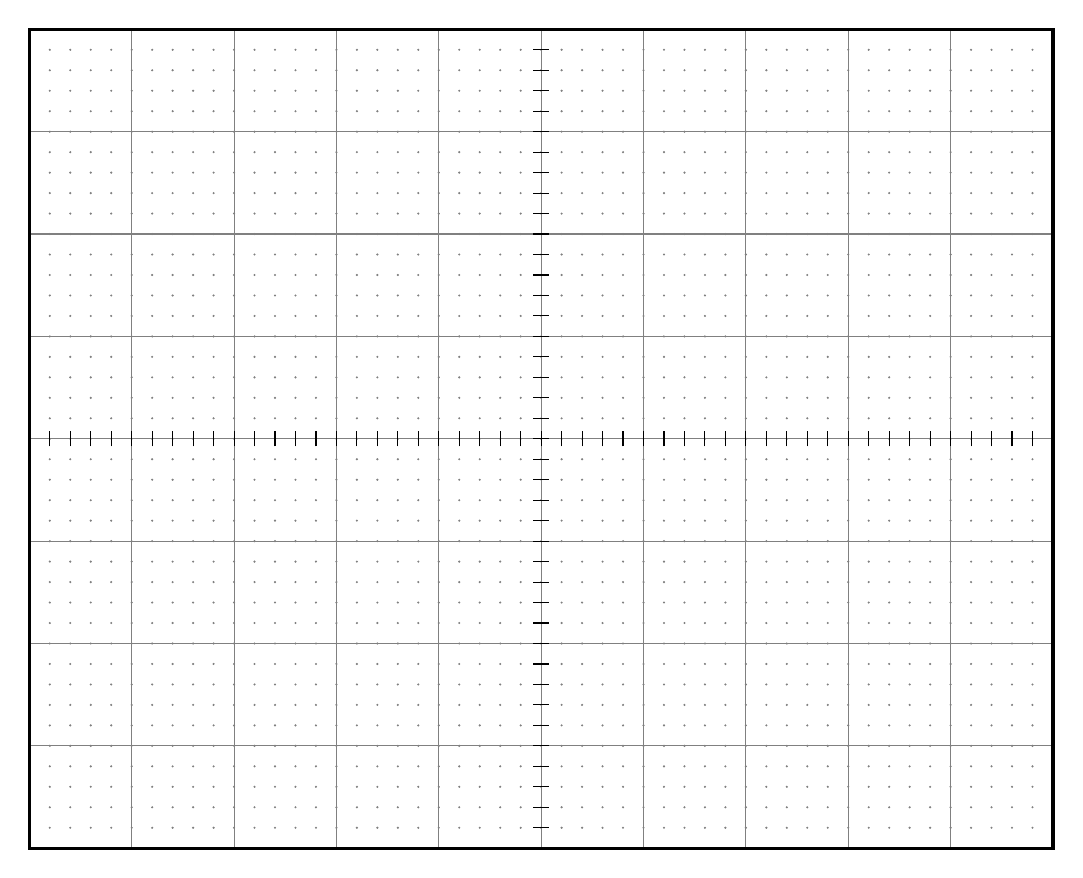
\begin{tikzpicture}
    % Define dimensions
    \def\gridwidth{10}
    \def\gridheight{8}
    \def\spacing{1.3}
    % Draw grid paper on the left
    \begin{scope}[xshift=0cm, yshift=0cm]
        % Grid points
        \foreach \x in {0,2,...,100}
        {
            \foreach \y in {0,2,...,80}
            {
                \draw[gray, fill=gray] (\x*\spacing/10, \y*\spacing/10) circle (0.05mm);
            }
        }
        % Major grid lines
        \foreach \x in {0,1,...,\gridwidth}
            \draw[gray] (\x*\spacing,0) -- (\x*\spacing,\gridheight*\spacing);
        \foreach \y in {0,1,...,\gridheight}
            \draw[gray] (0,\y*\spacing) -- (\gridwidth*\spacing,\y*\spacing);
        \draw[black, very thick] (0,0) rectangle (\gridwidth*\spacing,\gridheight*\spacing);
        % Center gridlines
        \foreach \x in {0,2,...,100}
            \draw (\x*\spacing/10, 3.925*\spacing) -- (\x*\spacing/10, 4.075*\spacing);
        \foreach \y in {0,2,...,80}
            \draw (4.925*\spacing, \y*\spacing/10) -- (5.075*\spacing, \y*\spacing/10);
    \end{scope}
\end{tikzpicture}
    \end{center}

    Compute the expected value of $\tau$ below, and use the plot to estimate the time constant.

    \begin{center}
        \renewcommand{\arraystretch}{2}
        \begin{tabular}{lp{2cm}clp{2cm}clp{3cm}}
            $R=$ & & & $C=$ & & & $RC=$ &
            \\
            \cline{2-2}\cline{5-5}\cline{8-8}
            \multicolumn{6}{l}{Time of charging to within $1/e$ of max. value of $V_C$} & &
            \\
            \cline{8-8}
            \multicolumn{6}{l}{Time of discharging to within $1/e$ of min. value of $V_C$} & &
            \\
            \cline{8-8}
            \multicolumn{6}{r}{Average} & &
            \\
            \cline{8-8}
        \end{tabular}
    \end{center}

    %%% Change R or C by 30%
    \filbreak
    \question[1] \textbf{30\% values data}: change either $R$ or $C$ by 30\% and sketch the resulting pattern in Graph~\ref{graph: rc scope trace 2}.

    \begin{center}
    \captionsetup{font=normalsize}
    \captionof{graph}{RC charge and discharge pattern for $R$ or $C$ adjusted by 30\%. \label{graph: rc scope trace 2}}
    % Oscilloscope grid
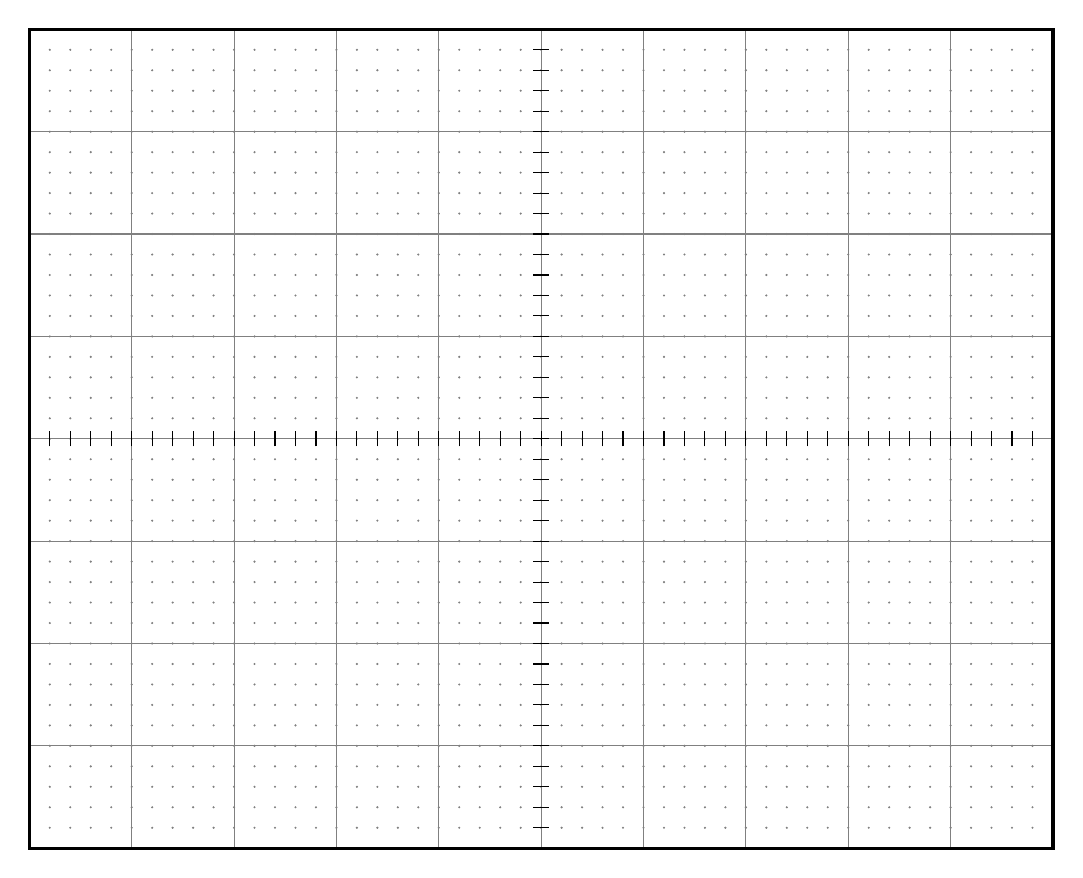
\begin{tikzpicture}
    % Define dimensions
    \def\gridwidth{10}
    \def\gridheight{8}
    \def\spacing{1.3}
    % Draw grid paper on the left
    \begin{scope}[xshift=0cm, yshift=0cm]
        % Grid points
        \foreach \x in {0,2,...,100}
        {
            \foreach \y in {0,2,...,80}
            {
                \draw[gray, fill=gray] (\x*\spacing/10, \y*\spacing/10) circle (0.05mm);
            }
        }
        % Major grid lines
        \foreach \x in {0,1,...,\gridwidth}
            \draw[gray] (\x*\spacing,0) -- (\x*\spacing,\gridheight*\spacing);
        \foreach \y in {0,1,...,\gridheight}
            \draw[gray] (0,\y*\spacing) -- (\gridwidth*\spacing,\y*\spacing);
        \draw[black, very thick] (0,0) rectangle (\gridwidth*\spacing,\gridheight*\spacing);
        % Center gridlines
        \foreach \x in {0,2,...,100}
            \draw (\x*\spacing/10, 3.925*\spacing) -- (\x*\spacing/10, 4.075*\spacing);
        \foreach \y in {0,2,...,80}
            \draw (4.925*\spacing, \y*\spacing/10) -- (5.075*\spacing, \y*\spacing/10);
    \end{scope}
\end{tikzpicture}
    \end{center}

    Compute the expected value of $\tau$ below, and use the plot to estimate the time constant.

    \begin{center}
        \renewcommand{\arraystretch}{2}
        \begin{tabular}{lp{2cm}clp{2cm}clp{3cm}}
            $R=$ & & & $C=$ & & & $RC=$ &
            \\
            \cline{2-2}\cline{5-5}\cline{8-8}
            \multicolumn{6}{l}{Time of charging to within $1/e$ of max. value of $V_C$} & &
            \\
            \cline{8-8}
            \multicolumn{6}{l}{Time of discharging to within $1/e$ of min. value of $V_C$} & &
            \\
            \cline{8-8}
            \multicolumn{6}{r}{Average} & &
            \\
            \cline{8-8}
        \end{tabular}
    \end{center}

    %%% Unknown capacitance
    \filbreak
    \question \textbf{Unknown capacitance data}:
    
    \begin{parts}

        \part[\half] Swap in an unknown $C$ and sketch the resulting pattern in Graph~\ref{graph: rc scope trace 3}.

        \begin{center}
        \captionsetup{font=normalsize}
        \captionof{graph}{RC charge and discharge pattern for unknown capacitance $C$. \label{graph: rc scope trace 3}}
        % Oscilloscope grid
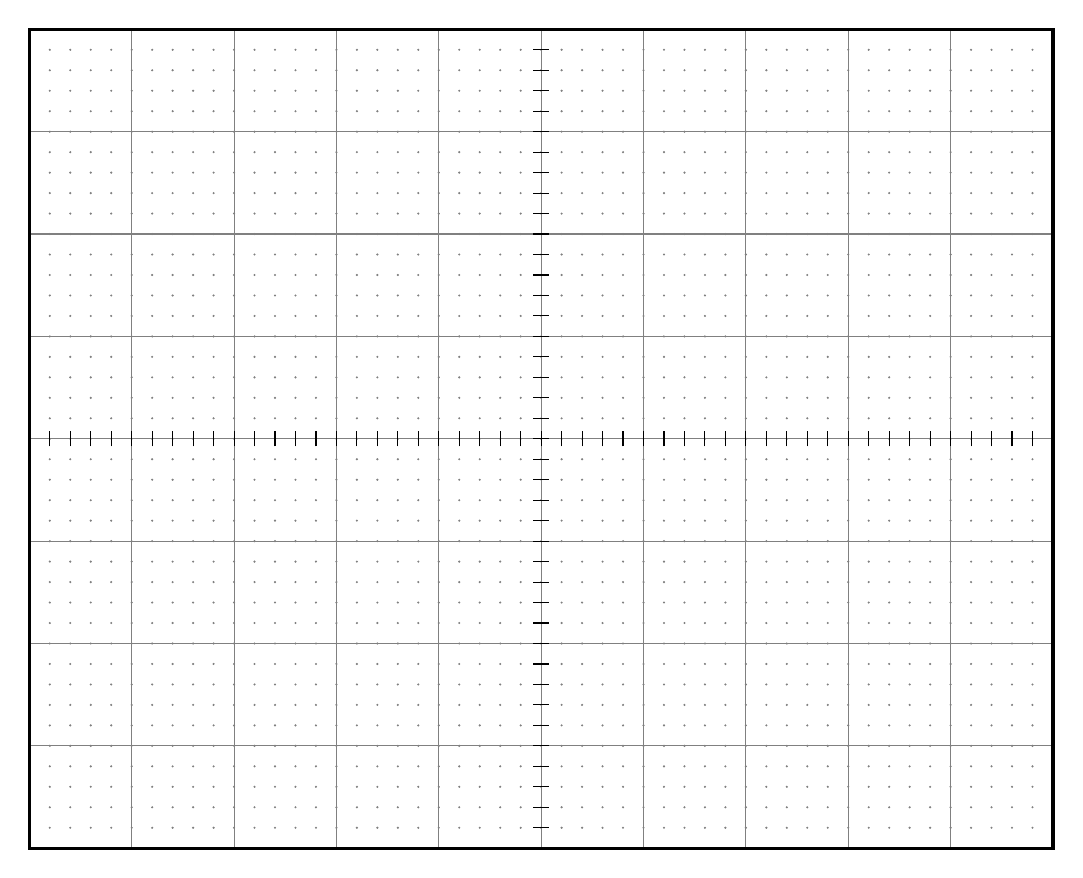
\begin{tikzpicture}
    % Define dimensions
    \def\gridwidth{10}
    \def\gridheight{8}
    \def\spacing{1.3}
    % Draw grid paper on the left
    \begin{scope}[xshift=0cm, yshift=0cm]
        % Grid points
        \foreach \x in {0,2,...,100}
        {
            \foreach \y in {0,2,...,80}
            {
                \draw[gray, fill=gray] (\x*\spacing/10, \y*\spacing/10) circle (0.05mm);
            }
        }
        % Major grid lines
        \foreach \x in {0,1,...,\gridwidth}
            \draw[gray] (\x*\spacing,0) -- (\x*\spacing,\gridheight*\spacing);
        \foreach \y in {0,1,...,\gridheight}
            \draw[gray] (0,\y*\spacing) -- (\gridwidth*\spacing,\y*\spacing);
        \draw[black, very thick] (0,0) rectangle (\gridwidth*\spacing,\gridheight*\spacing);
        % Center gridlines
        \foreach \x in {0,2,...,100}
            \draw (\x*\spacing/10, 3.925*\spacing) -- (\x*\spacing/10, 4.075*\spacing);
        \foreach \y in {0,2,...,80}
            \draw (4.925*\spacing, \y*\spacing/10) -- (5.075*\spacing, \y*\spacing/10);
    \end{scope}
\end{tikzpicture}
        \end{center}
    
        \begin{center}
            \renewcommand{\arraystretch}{2}
            \begin{tabular}{lp{2cm}clp{2cm}clp{3cm}}
                $R=$ & & & $C=$ & \textbf{unknown} & & $RC=$ & \textbf{unknown}
                \\
                \cline{2-2}\cline{5-5}\cline{8-8}
                \multicolumn{6}{l}{Time of charging to within $1/e$ of max. value of $V_C$} & &
                \\
                \cline{8-8}
                \multicolumn{6}{l}{Time of discharging to within $1/e$ of min. value of $V_C$} & &
                \\
                \cline{8-8}
                \multicolumn{6}{r}{Average} & &
                \\
                \cline{8-8}
            \end{tabular}
        \end{center}

        \begin{solution}[1cm]
            
        \end{solution}
    
        \part[\half] Calculate the unknown capacitance from your measured value of $RC$.
        %
        \begin{solution}[2cm]
            
        \end{solution}

    \end{parts}

    %%% Unknown resistance
    \filbreak
    \question \textbf{Unknown resistance data}:
    
    \begin{parts}

        \part[\half] Swap in an unknown $R$ and sketch the resulting pattern in Graph~\ref{graph: rc scope trace 4}.

        \begin{center}
        \captionsetup{font=normalsize}
        \captionof{graph}{RC charge and discharge pattern for unknown resistor $R$. \label{graph: rc scope trace 4}}
        % Oscilloscope grid
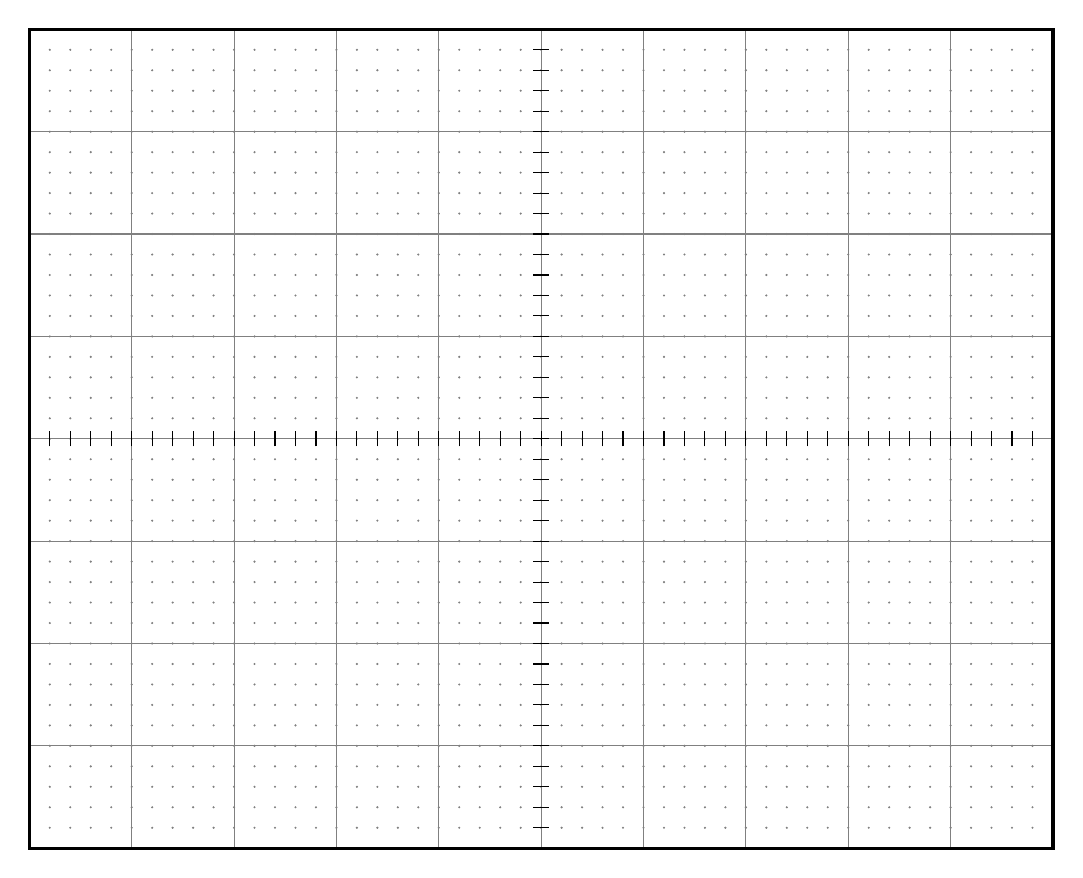
\begin{tikzpicture}
    % Define dimensions
    \def\gridwidth{10}
    \def\gridheight{8}
    \def\spacing{1.3}
    % Draw grid paper on the left
    \begin{scope}[xshift=0cm, yshift=0cm]
        % Grid points
        \foreach \x in {0,2,...,100}
        {
            \foreach \y in {0,2,...,80}
            {
                \draw[gray, fill=gray] (\x*\spacing/10, \y*\spacing/10) circle (0.05mm);
            }
        }
        % Major grid lines
        \foreach \x in {0,1,...,\gridwidth}
            \draw[gray] (\x*\spacing,0) -- (\x*\spacing,\gridheight*\spacing);
        \foreach \y in {0,1,...,\gridheight}
            \draw[gray] (0,\y*\spacing) -- (\gridwidth*\spacing,\y*\spacing);
        \draw[black, very thick] (0,0) rectangle (\gridwidth*\spacing,\gridheight*\spacing);
        % Center gridlines
        \foreach \x in {0,2,...,100}
            \draw (\x*\spacing/10, 3.925*\spacing) -- (\x*\spacing/10, 4.075*\spacing);
        \foreach \y in {0,2,...,80}
            \draw (4.925*\spacing, \y*\spacing/10) -- (5.075*\spacing, \y*\spacing/10);
    \end{scope}
\end{tikzpicture}
        \end{center}
    
        \begin{center}
            \renewcommand{\arraystretch}{2}
            \begin{tabular}{lp{2cm}clp{2cm}clp{3cm}}
                $R=$ & \textbf{unknown} & & $C=$ & & & $RC=$ & \textbf{unknown}
                \\
                \cline{2-2}\cline{5-5}\cline{8-8}
                \multicolumn{6}{l}{Time of charging to within $1/e$ of max. value of $V_C$} & &
                \\
                \cline{8-8}
                \multicolumn{6}{l}{Time of discharging to within $1/e$ of min. value of $V_C$} & &
                \\
                \cline{8-8}
                \multicolumn{6}{r}{Average} & &
                \\
                \cline{8-8}
            \end{tabular}
        \end{center}

        \begin{solution}[1cm]
            
        \end{solution}
    
        \part[\half] Calculate the unknown resistance from your measured value of $RC$.
        %
        \begin{solution}[2cm]
            
        \end{solution}

    \end{parts}

    \filbreak
    \question[2] What systematic or random errors can you think of that might account for differences between the measured and calculated values of the time constant? List at least two.
    %
    \begin{solution}[2cm]
        
    \end{solution}

    \filbreak
    \question[2] How accurately do you think you can measure a time constant from your traces of the oscilloscope pattern? Justify your answer.
    %
    \begin{solution}[2cm]
        
    \end{solution}

    \endgradingrange{rc}

    %%% RLC Circuit
    \fullwidth{\subsection*{RLC Resonant Circuit (\pointsinrange{rlc} points)}}

    \begingradingrange{rlc}

    \filbreak
    \question[3] Enter your measurements in Data Table~\ref{data: rlc circuit}:

    \begin{center}
        \renewcommand{\arraystretch}{2}
        \begin{tabular}{lp{2cm}clp{2cm}clp{3cm}}
            $L=$ & & & $C=$ & & & $f_0=$ & 
            \\
            \cline{2-2}\cline{5-5}\cline{8-8}
        \end{tabular}
    \end{center}

    \begin{center}
        \captionsetup{font=normalsize}
        \captionof{data table}{Response function measurements of the RLC circuit. \label{data: rlc circuit}}
        \renewcommand{\arraystretch}{1.5}
        \begin{tabular}{|>{\centering\arraybackslash}p{2cm}|>{\centering\arraybackslash}p{2cm}|p{0.25cm}|>{\centering\arraybackslash}p{2cm}|>{\centering\arraybackslash}p{2cm}|p{0.25cm}|>{\centering\arraybackslash}p{2cm}|>{\centering\arraybackslash}p{2cm}|}
        \cline{1-2}\cline{4-5}\cline{7-8}
        \multicolumn{2}{|c|}{$R=\qty{400}{\ohm}$} &  & \multicolumn{2}{|c|}{$R=\qty{200}{\ohm}$} &  & \multicolumn{2}{|c|}{$R=\qty{100}{\ohm}$}
        \\
        \cline{1-2}\cline{4-5}\cline{7-8}
        Frequency $f$ (Hz)       & Voltage $V_R$ (V)      &  & Frequency $f$ (Hz)       & Voltage $V_R$ (V)      &  & Frequency $f$ (Hz)       & Voltage $V_R$ (V)
        \\
        \cline{1-2}\cline{4-5}\cline{7-8}
                             &                  &  &                      &                  &  &                      &                  
        \\
        \cline{1-2}\cline{4-5}\cline{7-8}
                             &                  &  &                      &                  &  &                      &                 
        \\
        \cline{1-2}\cline{4-5}\cline{7-8}
                             &                  &  &                      &                  &  &                      &                 
        \\
        \cline{1-2}\cline{4-5}\cline{7-8}
                             &                  &  &                      &                  &  &                      &                 
        \\
        \cline{1-2}\cline{4-5}\cline{7-8}
                             &                  &  &                      &                  &  &                      &                 
        \\
        \cline{1-2}\cline{4-5}\cline{7-8}
                             &                  &  &                      &                  &  &                      &                 
        \\
        \cline{1-2}\cline{4-5}\cline{7-8}
                             &                  &  &                      &                  &  &                      &                 
        \\
        \cline{1-2}\cline{4-5}\cline{7-8}
                             &                  &  &                      &                  &  &                      &                 
        \\
        \cline{1-2}\cline{4-5}\cline{7-8}
                             &                  &  &                      &                  &  &                      &                 
        \\
        \cline{1-2}\cline{4-5}\cline{7-8}
                             &                  &  &                      &                  &  &                      & 
        \\
        \cline{1-2}\cline{4-5}\cline{7-8}
        \end{tabular}
    \end{center}

    \filbreak
    \question[3] Plot resistor voltage $V_R$ versus frequency $f$ for all three values of $R$ in Graph~\ref{graph: rlc responses}, using solid circles for $R=\qty{400}{\ohm}$, hollow squares for $R=\qty{200}{\ohm}$, and small x's for $R=\qty{100}{\ohm}$. Interpolate between the points in each separate set to produce smooth curves. You should find that $R=\qty{400}{\ohm}$ produces the broadest response.

    \begin{center}
    \captionsetup{font=normalsize}
    \captionof{graph}{Response function of the $RLC$ circuit. \label{graph: rlc responses}}
    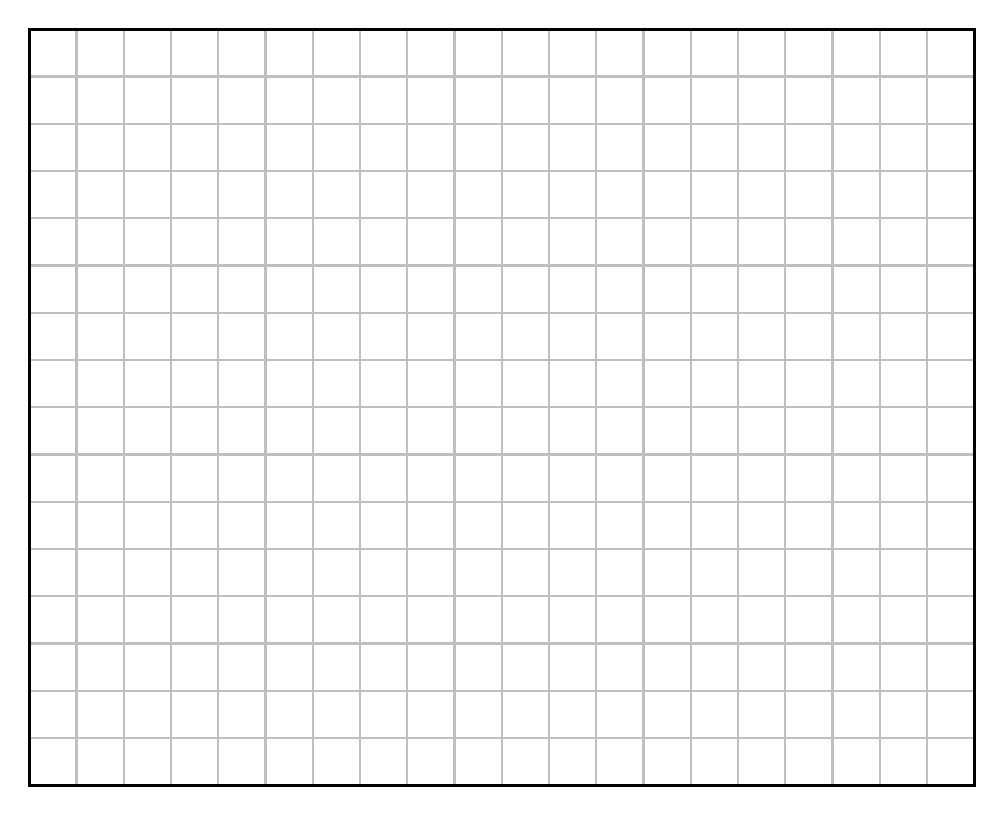
\begin{tikzpicture}
        % Define dimensions
        \def\gridwidth{20}
        \def\gridheight{16}
        \def\spacing{0.6}
        % Draw grid paper on the left
        \begin{scope}[xshift=0cm,yshift=0cm]
            % Major grid lines (thicker)
            \foreach \x in {0,1,...,\gridwidth}
                \draw[gray!50,thick] (\x*\spacing,0) -- (\x*\spacing,\gridheight*\spacing);
            \foreach \y in {0,1,...,\gridheight}
                \draw[gray!50, thick] (0,\y*\spacing) -- (\gridwidth*\spacing,\y*\spacing);
            \draw[black, very thick] (0,0) rectangle (\gridwidth*\spacing,\gridheight*\spacing);
        \end{scope}
    \end{tikzpicture}
    \end{center}

    \filbreak
    \question[1] How do the resonant frequencies compare in the three response functions? Is this expected? Explain.
    %
    \begin{solution}[3cm]
        
    \end{solution}

    \filbreak
    \question[1] From your plots, measure the $Q$ factor for each of the three curves, showing your work for at least one of the three values. Use $Q=f_0/\Delta f$ from eq.~\ref{eq: Q factor} to compute $Q$.
    %
    \begin{solution}[3cm]
        
    \end{solution}

    \filbreak
    \question[1] Calculate $Q$ for each of the three values of $R$ used (\qty{100}{\ohm}, \qty{200}{\ohm}, and \qty{400}{\ohm}) using
    \[
        Q = \frac{1}{R}\sqrt{\frac{L}{C}}
    \]
    from eq.~\ref{eq: Q factor}. Show your work for at least one of the three calculations.
    %
    \begin{solution}[6cm]
        
    \end{solution}

    \filbreak
    \question[2] Using the values of $Q$ that you measured from the plots of the response function, plot $1/Q$ versus $R$ in Graph~\ref{graph: 1/Q vs R} below.

    \begin{center}
    \captionsetup{font=normalsize}
    \captionof{graph}{Plot of $1/Q$ versus $R$. \label{graph: 1/Q vs R}}
    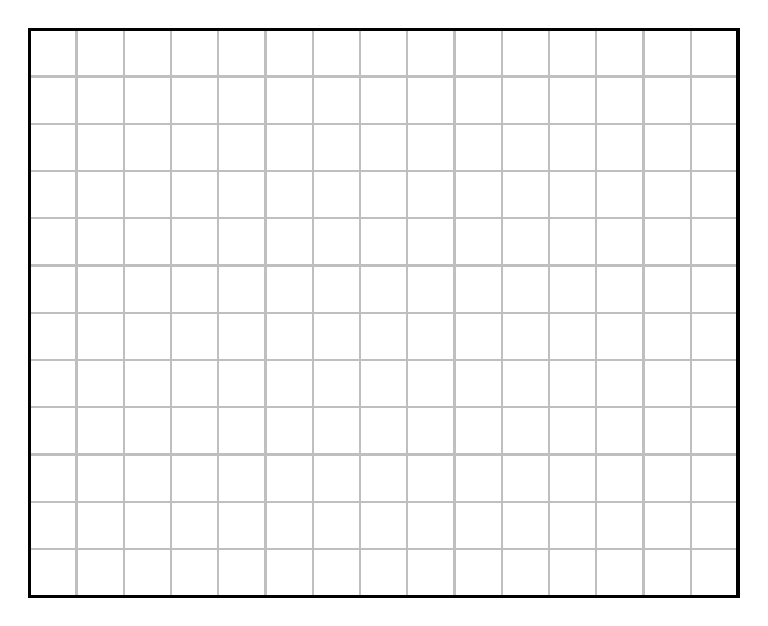
\begin{tikzpicture}
        % Define dimensions
        \def\gridwidth{15}
        \def\gridheight{12}
        \def\spacing{0.6}
        % Draw grid paper on the left
        \begin{scope}[xshift=0cm,yshift=0cm]
            % Major grid lines (thicker)
            \foreach \x in {0,1,...,\gridwidth}
                \draw[gray!50,thick] (\x*\spacing,0) -- (\x*\spacing,\gridheight*\spacing);
            \foreach \y in {0,1,...,\gridheight}
                \draw[gray!50, thick] (0,\y*\spacing) -- (\gridwidth*\spacing,\y*\spacing);
            \draw[black, very thick] (0,0) rectangle (\gridwidth*\spacing,\gridheight*\spacing);
        \end{scope}
    \end{tikzpicture}
    \end{center}

    Does the plot of $1/Q$ versus $R$ look like a straight line, as you would expect from eq.~\ref{eq: Q factor}? Draw a best-fit line and measure the slope. How close is your slope to its expected value?
    
    \endgradingrange{rlc}

\end{postlab}

\end{document}